\section{Perspective and vanishing point}

If we opt to consider all lines parallel to the direction parameters $\begin{bmatrix} \alpha & \beta & 1 \end{bmatrix}$, we can establish the following system of equations:
\[
    \begin{cases}
        X = X_0 + \alpha Z  \\
        Y = Y_0 + \beta Z   \\
        Z = 1 \cdot Z
    \end{cases}
\]
To project these lines onto the 2D image using the triangle equality, we derive the following expressions:
\[x=f \dfrac{X}{Z} = f \dfrac{X_0 + \alpha Z}{Z} = f\alpha + \dfrac{X_0}{Z}\]
\[y=f \dfrac{Y}{Z} = f \dfrac{Y_0 + \beta Z}{Z}  = f\beta  + \dfrac{Y_0}{Z}\]
Now, let's find the image of the point at infinity along these lines, which yields the point:
\[\begin{bmatrix} f\alpha & f\beta \end{bmatrix}\]
Remarkably, this image point is independent of the values of $X_0$ and $Y_0$. 
Hence, all parallel lines share the same image of their points at infinity.
\newpage
\begin{definition}
    The image of the point at the infinity of the lines is known as the \emph{vanishing point}. 
\end{definition}
As a result, we observe that all lines parallel in the real world project onto converging lines in the image.
\begin{figure}[H]
    \centering
    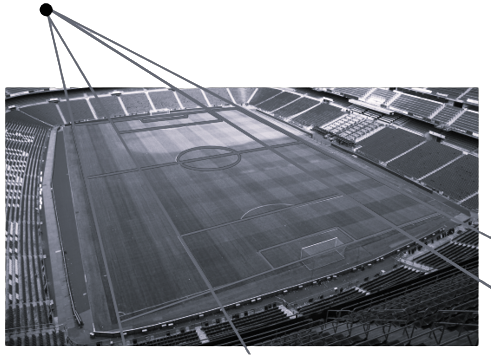
\includegraphics[width=0.4\linewidth]{images/vanishingpoint.png}
    \caption{Example of vanishing point}
\end{figure}